\section{Example}

For links see \hyperlink{target}{the aptly named chapter at the end}.

\subsection{Citations}
\label{subsec:citations}

\subparagraph{Citations} are very important like for a book\footcite{SJGTHS:1} or for a website\footcite{COADE:1}. You find them in the \emph{citations.bib} file.

\subsection{Figures}

\begin{figure}[H]
	\centering
	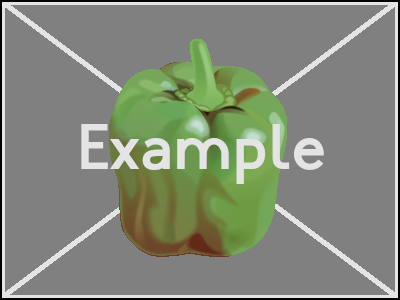
\includegraphics[width=\textwidth]{res/example.png}
	\caption[Short caption]{One figure centered full width}
	\label{fig:bigImage}
\end{figure}

\begin{figure}[H]
	\centering
	\begin{minipage}[b]{0.45\textwidth}
		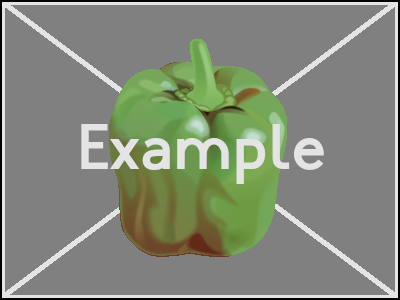
\includegraphics[width=\textwidth]{res/example.png}
		\caption{Left figure}
	\end{minipage}
	\hfill
	\begin{minipage}[b]{0.45\textwidth}
		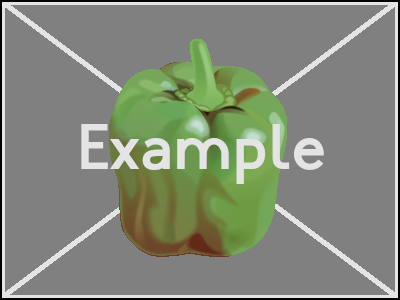
\includegraphics[width=\textwidth]{res/example.png}
		\caption{Right figure}
	\end{minipage}
\end{figure}

Notice how we can setup a \emph{label} and then reference the figure \ref{fig:bigImage} on page \pageref{fig:bigImage} with the \emph{ref} command.

\subsection{Tables}

\begin{table}[H]
	\centering
	\resizebox{\textwidth}{!}{ % this neat trick will resize the table down
	\begin{tabular}{ || m{3cm} | m{5cm} | m{8cm} || }
		\hline
		\textbf{A title} & \textbf{B title} & \textbf{C title} \\
		\hline
		\hline
		A & B & C\\
		\hline
		A & B & C\\
		\hline
		A & B & C\\
		\hline
	\end{tabular}
	}
	\caption{Simple table with lines}
	\label{tab:exampleTable}
\end{table}

\subsection{Lists, Bulletpoints and Enumerations}

This itemize list is default.
\begin{itemize}
	\item A
	\item B
	\item C
\end{itemize}

This enumerate list has \emph{noitemsep} added.
\begin{enumerate}[noitemsep]
	\item A
	\item B
	\item C
\end{enumerate}

\hypertarget{target}{\subsection{Links and References}}

A label works great to reference something inside the document like section~\ref{subsec:citations} the citations on page~\pageref{subsec:citations}.\\
For more freedom to navigate consider a hypertarget and hyperlink like this chapter title.
For external webpages use \url{https://en.wikibooks.org/wiki/LaTeX/Labels_and_Cross-referencing} but a citation would be better suited most of the time.

\subsection{Glossary}
This is a \gls{test} if the glossaries package works as expected.
Remember that in TeXstudio you have to generate the glossary with F9 (makeglossaries command) first before it will show up.